% ===========================================================================
% Article B (technological / exploratory): Twin arithmetic as a domain selector
% Narrative arc: antecedents -> general toolkit -> generalization -> simulations
% ===========================================================================
\documentclass[11pt,a4paper]{article}
\usepackage[utf8]{inputenc}
\usepackage[T1]{fontenc}
\usepackage{lmodern}
\usepackage[english]{babel}
\usepackage{amsmath,amssymb,amsthm,amsfonts}
\usepackage{booktabs}
\usepackage{graphicx}
\usepackage{listings}
\usepackage[margin=1in]{geometry}
\usepackage{xcolor}
\usepackage{hyperref}
\hypersetup{colorlinks=true, linkcolor=blue!60!black, citecolor=blue!50!black,
            urlcolor=blue!60!black}

\newcommand{\Op}{\mathrm{Op}}
\newcommand{\R}{\mathbb{R}}
\newcommand{\C}{\mathbb{C}}
\newcommand{\Z}{\mathbb{Z}}
\newcommand{\code}[1]{\texttt{#1}}

\lstset{basicstyle=\ttfamily\small, columns=fullflexible,
        keywordstyle=\color{blue!60!black}, commentstyle=\color{green!40!black},
        showstringspaces=false, language=Python, frame=single,
        rulecolor=\color{black!25}, breaklines=true}

\theoremstyle{definition}
\newtheorem{remark}{Remark}

\title{\textbf{Twin Arithmetic as a Computational-Domain Selector}\\[0.3em]
\large From the Log-Domain Trick to a Measured, General Toolkit}
\author{Jocelyn Nemb\'e\\
\small Modeling and Calculus Laboratory, National Institute of Management
Sciences, Libreville, Gabon\\
\small ROOTS-INSIGHTS \quad\textbar\quad \texttt{jnembe@roots-insights.org}}
\date{June 2026}

\begin{document}
\maketitle

\begin{abstract}
\noindent
Scientific computing already exploits deformed arithmetic ad hoc: log-domain
likelihoods, the stable log-sum-exp, multiplicative calculus in finance, and
log--log linearization. We show these are all instances of one construction ---
the twin reduction $\bigoplus_\varphi x_i=\varphi^{-1}(\sum_i\varphi(x_i))$ for a
generator $\varphi$ --- and we build a reproducible symbolic--numeric toolkit
that \emph{generates} any such domain in four formats (SymPy, \LaTeX, Unicode,
mpmath) and \emph{measures} the cost of a task in each. We then generalize:
the same machine selects, by evidence rather than convention, the optimal base
for a given task, and extends to one-parameter Lie and compact-Lie ($SU(n)$)
domains. Simulations quantify the gains against existing practice: the
transformed domain is exact where the original underflows (log-likelihood),
matches the stable log-sum-exp (softmax), and automates optimal-base selection
(power $\to$ log--log, exponential $\to$ semi-log), with an explicit
speed/stability trade-off. We close with exploratory directions --- qudit-gate
universality, operational cryptography, primary-decomposition compression ---
separating measured facts from speculation. The library carries $131$ passing
tests.
\end{abstract}

\noindent\textbf{Keywords:} log-domain computation, log-sum-exp, non-Newtonian
calculus, numerical stability, optimal base selection, symbolic--numeric
software.

\section{Introduction}

This paper follows the same four-movement arc as its scientific companion, in a
technological key. We (1) recall the established deformed-arithmetic techniques
of scientific computing and what they buy; (2) place them inside the general
twin construction; (3) generalize them into a single toolkit that generates and
\emph{measures} arbitrary computational domains; and (4) report simulations that
compare the generalization against existing practice. The thesis is concrete:
\emph{the group element is the computational domain, and choosing it well is a
measurable decision.}

\section{Antecedents in scientific computing}
\label{sec:prior}

\paragraph{Log-domain computation.} Probabilistic and statistical codes
routinely work with log-likelihoods $\sum_i\log p_i$ rather than products
$\prod_i p_i$, because the product underflows; hidden-Markov inference and
Viterbi decoding run in the log domain for the same reason. The stable
\emph{log-sum-exp}, $\mathrm{LSE}(z)=\log\sum_i e^{z_i}$ computed with a
max-shift, underlies softmax and partition-function evaluation \cite{blanchard}.
These techniques buy dynamic range and stability, but are applied as
domain-specific folklore.

\paragraph{Multiplicative / geometric calculus.} Grossman--Katz calculus
\cite{grossman} and its geometric variant are used in growth modelling, finance,
and image processing, where multiplicative structure is native. The contribution
is a calculus matched to the data's symmetry.

\paragraph{Linearization.} Log--log and semi-log plots, and the link functions
of generalized linear models, linearize power laws and exponentials before
fitting --- a manual choice of representation that is, again, a base selection.

\section{The general toolkit}
\label{sec:toolkit}

All three antecedents are the twin reduction of a generator $\varphi$:
\begin{equation}\label{eq:reduce}
\bigoplus_\varphi x_i=\varphi^{-1}\!\Bigl(\textstyle\sum_i\varphi(x_i)\Bigr),
\qquad T:=\sum_i\varphi(x_i)\ \text{(transformed total).}
\end{equation}
For $\varphi=\mathrm{id}$ this is summation; for $\varphi=\log$ the product, with
$T$ the log-likelihood; for $\varphi=\exp$ the log-sum-exp. The toolkit
\code{arithmetics.symbolic.twin} (SymPy, NumPy, mpmath) generates these
operations symbolically in four formats and bridges to numerics; it is layered
(Table~\ref{tab:arch}) with per-layer unit tests.

\begin{lstlisting}
from arithmetics.symbolic.twin import BijectionAction, twin_operation
phi = BijectionAction.exponential()
twin_operation(phi, -1, "add").text()   # 'x*y'       (multiplication)
twin_operation(phi,  1, "add").text()   # 'log(exp(x) + exp(y))'  (log-sum-exp)
\end{lstlisting}

\begin{table}[ht]
\centering
\caption{Layered architecture of the toolkit
(module \code{arithmetics.symbolic.twin}).}
\label{tab:arch}
\begin{tabular}{ll}
\toprule
layer & contents \\
\midrule
symbolic engine & transfers, level-$p$ ops, defect, $\zeta_p$ (SymPy/\LaTeX/Unicode/mpmath) \\
twin generator & transport; monogenic, one-parameter Lie, finite actions \\
compact Lie & $SO(2),SO(3),SU(2),SU(n)$ with Haar sampling \\
decision & class equation, normalizer orbits, $SU(2)$ Weyl \\
primary decomposition & abelian $\Op\cong\prod_p\Op_p$ \\
arithmetic-task costs & domain selection, optimal base, op counts \\
qudits & $SU(n)$ Weyl integration, Schur characters \\
\bottomrule
\end{tabular}
\end{table}

\paragraph{Generalization.} Beyond reproducing the antecedents
(Table~\ref{tab:hier}), the toolkit (i) \emph{measures} the numerical cost of a
task in each domain so the base is chosen by evidence, and (ii) extends transport
to arbitrary one-parameter Lie and compact-Lie group actions. This converts
scattered folklore into a single, auditable selection procedure.

\begin{remark}[What changes]
The novelty is not a new arithmetic but a new \emph{discipline}: the
computational domain becomes a parameter that is generated symbolically and
chosen by measurement --- the way a numerical method is selected by its error
bound rather than by habit.
\end{remark}

\begin{table}[ht]
\centering
\caption{The exponential hierarchy, generated symbolically
($\odot_e=+$, $G=\langle\exp\rangle$).}
\label{tab:hier}
\begin{tabular}{rll}
\toprule
level $n$ & $x\odot_{en}y$ & name \\
\midrule
$0$  & $x+y$               & addition \\
$1$  & $\log(e^x+e^y)$     & log-sum-exp \\
$-1$ & $x\cdot y$          & multiplication \\
$-2$ & $x^{\ln y}$         & symmetric power \\
\bottomrule
\end{tabular}
\end{table}

\section{Simulations and comparison with practice}
\label{sec:sims}

\subsection{Domain of computation: the log-likelihood}

To evaluate $T=\sum_i\log x_i$ one may sum in the transformed domain or form the
product first and take its log. On wide-range data the product underflows
($\log 0=-\infty$); the transformed domain is exact to rounding.
Figure~\ref{fig:logdomain} measures the relative error of both against a
$60$-digit reference as the number of factors grows; Table~\ref{tab:measured}
reports a representative run. \emph{Comparison:} this is the standard log-domain
trick, here \emph{quantified} (the underflow threshold) and \emph{automated} by a
pre-computation rule that reads the data's dynamic range.

\begin{figure}[ht]
\centering
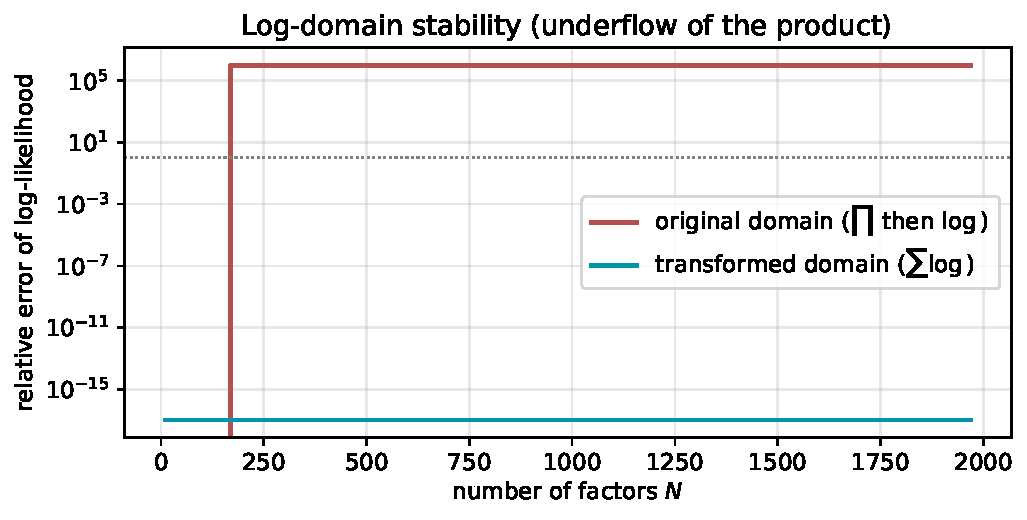
\includegraphics[width=0.76\textwidth]{figures/B1_logdomain.pdf}
\caption{Log-likelihood: the original domain (product then log) underflows; the
transformed domain ($\sum\log$) stays at machine precision.}
\label{fig:logdomain}
\end{figure}

\noindent\emph{Reading.} The curves cross from ``both fine'' to ``only the log
domain works'' at the underflow threshold. The lesson is not that one domain is
always better, but that the threshold is \emph{predictable} from the data, so the
domain can be fixed before any arithmetic is done.

\begin{table}[ht]
\centering
\caption{Measured costs for a log-likelihood of $800$ probabilities spanning
$7.9$ decades ($\varphi=\log$).}
\label{tab:measured}
\begin{tabular}{lc}
\toprule
quantity & value \\
\midrule
dynamic range & $7.9$ decades \\
pre-computation recommendation & \code{transformed} \\
relative error, original domain & $\infty$ (product underflows) \\
relative error, transformed domain & $0$ \\
transcendental calls (naive\,/\,transformed) & $2397\,/\,801$ \\
\bottomrule
\end{tabular}
\end{table}

\subsection{A second domain: softmax / log-sum-exp}

The dual generator $\varphi=\exp$ gives the reduction
$\mathrm{LSE}(z)=\log\sum_i e^{z_i}=\bigoplus_{\exp}z_i$. Evaluated naively it
overflows for large $z_i$; the max-shifted form is stable.
Figure~\ref{fig:lse} measures both against a high-precision reference: the naive
log-sum-exp diverges, the shifted domain holds. \emph{Comparison:} the toolkit
recognizes the stable softmax of deep learning as the \emph{same} construction
\eqref{eq:reduce} for $\varphi=\exp$, unifying two folklore tricks under one
rule.

\begin{figure}[ht]
\centering
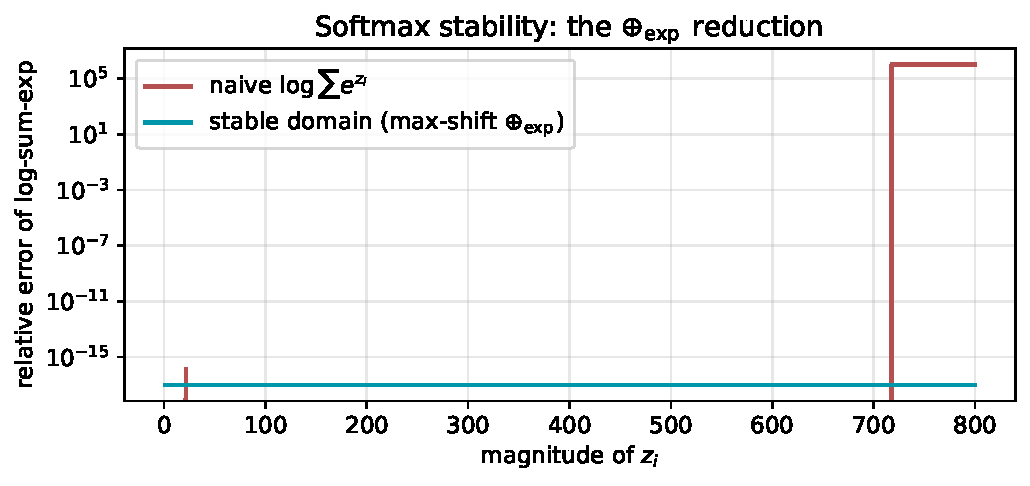
\includegraphics[width=0.76\textwidth]{figures/B5_lse.pdf}
\caption{Softmax stability: the naive $\log\sum e^{z_i}$ overflows; the stable
$\oplus_{\exp}$ reduction (max-shift) is exact. Relative error vs magnitude of
$z_i$.}
\label{fig:lse}
\end{figure}

\noindent\emph{Reading.} This is the overflow mirror of Figure~\ref{fig:logdomain}:
the same failure mode in the dual domain $\varphi=\exp$. The two figures together
show that the log-likelihood and softmax tricks are not two recipes but one ---
choose the domain in which the reduction stays bounded.

\subsection{Optimal base selection}

For representation, the toolkit selects the base $\varphi$ minimizing the
back-transformed fit RMSE. Figure~\ref{fig:base} shows that a power law selects
log--log, an exponential semi-log, and a line the identity, each beating the
alternatives by $10$--$13$ orders of magnitude. \emph{Comparison:} where an
analyst manually picks a log--log axis, the tool \emph{derives} the optimal base
from the data, before fitting.

\begin{figure}[ht]
\centering
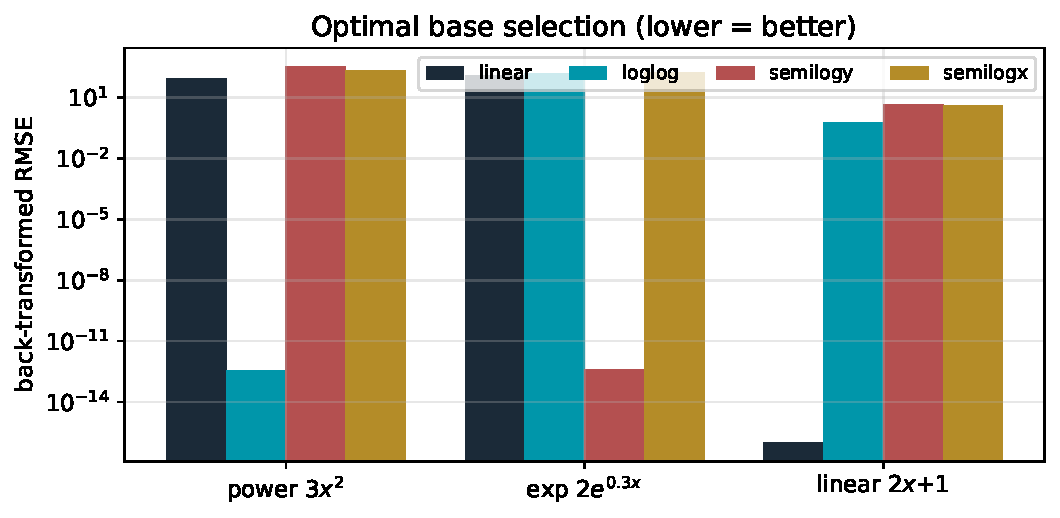
\includegraphics[width=0.80\textwidth]{figures/B2_optimal_base.pdf}
\caption{Optimal base selection: back-transformed RMSE per base (log scale); the
correct base wins decisively for each data type.}
\label{fig:base}
\end{figure}

\noindent\emph{Reading.} The $10$--$13$ order-of-magnitude gap between the best
and the runner-up base is what makes the choice unambiguous: the selector does
not need a fine tolerance to pick the right representation, only to read off the
clear minimum.

\begin{remark}[Why the optimal base wins decisively]\label{rem:why-base}
The order-of-magnitude gap of Figure~\ref{fig:base} is analytic, not incidental. A power law $y=ax^{b}$ becomes
\emph{exactly} affine in the log--log gauge, $\log y=\log a+b\log x$, so a linear fit there leaves only the noise
floor as residual and the back-transformed RMSE collapses to it; an exponential $y=ae^{bx}$ does the same in the
semi-log gauge $\log y=\log a+bx$. In \emph{any other} gauge the transformed data retain a nonzero curvature, so
the best affine fit keeps an irreducible $O(\text{curvature})$ residual. The selector therefore never weighs close
competitors: the correct gauge sits at the noise floor while every other sits at the curvature scale --- precisely
the $10$--$13$ decade separation observed.
\end{remark}

\subsection{The speed/stability trade-off}

Stability has a price. A generic twin-fold of $N$ items costs $3(N-1)$
transcendental calls; the batched transformed evaluation costs $N+1$
(Figure~\ref{fig:tradeoff}). The toolkit surfaces the trade-off so the choice is
explicit.

\begin{figure}[ht]
\centering
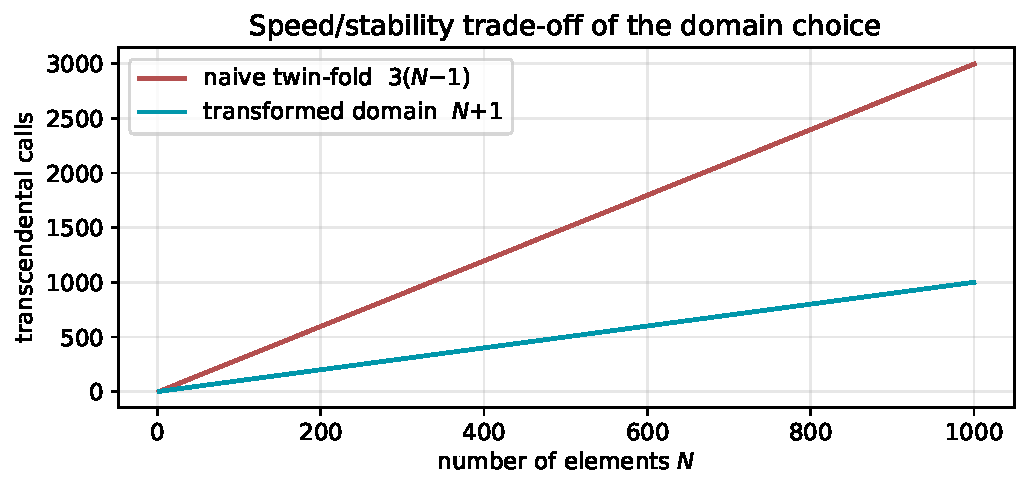
\includegraphics[width=0.70\textwidth]{figures/B3_tradeoff.pdf}
\caption{Transcendental-call counts for an $N$-element reduction: naive twin-fold
vs batched transformed domain.}
\label{fig:tradeoff}
\end{figure}

\noindent\emph{Reading.} Both costs are linear in $N$, so the domain choice
never changes the asymptotic complexity --- it is a constant-factor and a
stability decision, not an algorithmic one. The honest message is that stability
is bought, not free.

\subsection{Summary of the comparison}

Table~\ref{tab:compare} aligns each established technique with its twin-theoretic
view and the toolkit's contribution.

\begin{table}[ht]
\centering
\caption{Existing practice vs the general toolkit.}
\label{tab:compare}
\begin{tabular}{p{3.0cm}p{3.2cm}p{2.8cm}p{4.0cm}}
\toprule
task & conventional practice & twin view & toolkit contribution \\
\midrule
log-likelihood & ad hoc log domain & $\bigoplus_{\log}$, total $T$ &
measured threshold + pre-computation rule \\
softmax / partition & stable LSE (max-shift) & $\bigoplus_{\exp}$ &
unified as the same construction \\
power / exp fitting & manual log--log, semi-log & choose base $\varphi$ &
automated optimal-base selection \\
qudit gate analysis & CUE / Haar numerics & conjugation, $\Op\cong SU(d)$ &
universality measured (\S\ref{sec:explore}) \\
\bottomrule
\end{tabular}
\end{table}

\noindent\emph{Reading.} The third column shows the unification: four unrelated
techniques share one twin view. The fourth column shows the contribution: in
each case the toolkit replaces convention or folklore by a measured, automated
decision.

\section{Exploratory directions}
\label{sec:explore}

\paragraph{Qudit-gate universality (measured).} Under conjugation by $SU(d)$ a
generic bilinear gate on $\C^d$ has trivial structural kernel, so
$\Op\cong SU(d)$; linear operations are rigid. Figure~\ref{fig:univ} reports,
over Haar-sampled $SU(d)$, the fraction of elements preserving each operation:
$1$ for addition, $0$ for a generic gate, $d=2,\dots,6$. The fact is clean and
reproducible; its use for gate synthesis is open.

\begin{figure}[ht]
\centering
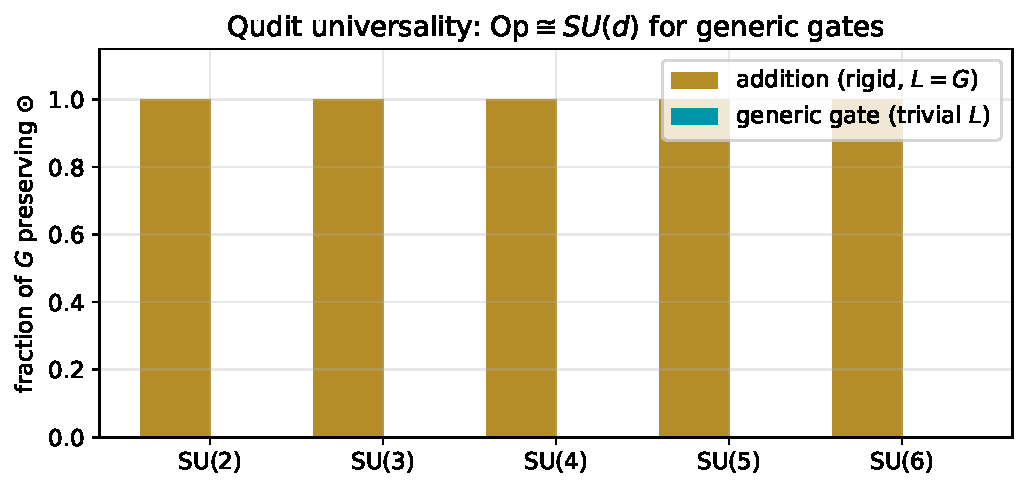
\includegraphics[width=0.72\textwidth]{figures/B4_universality.pdf}
\caption{Qudit universality: fraction of $SU(d)$ preserving the operation.
Addition is rigid; a generic gate has trivial kernel, so $\Op\cong SU(d)$.}
\label{fig:univ}
\end{figure}

\noindent\emph{Reading.} The two bar heights are the two extremes of the
linearity obstruction: $1$ means every symmetry preserves the operation (linear,
rigid), $0$ means none does (generic, maximally flexible). That the generic bar
stays at $0$ as $d$ grows is the qudit universality statement, read directly off
the simulation.

\paragraph{Operational cryptography (exploratory).} $\Op\cong G/L$ supports an
operational discrete-log problem whose hardness is bounded below by the
discrete log in $G/L$; its cryptographic value is open.

\paragraph{Compression via primary decomposition (exploratory).} For abelian
$G$, $\Op\cong\prod_p\Op_p$ suggests compact encodings of large operation
tables; the compression ratios remain to be benchmarked.

\section{Reproducibility}

The figures are regenerated by \code{papers/make\_figures.py} from the computed
data, with no synthetic inputs; the discovery tables are exported to
\code{results/twin/}; the test suite ($131$ tests) passes in full.

\section{Conclusion}

The deformed-arithmetic techniques scattered across scientific computing are one
construction in disguise. The toolkit makes that explicit, and --- the
technological payoff --- turns the choice of computational domain into a
\emph{measured} decision: generate the candidate arithmetics symbolically,
evaluate their real costs on the task, and select the base before computing. The
companion paper provides the group-theoretic discrimination theory; together
they render twin arithmetic a reproducible instrument.

\appendix

\section{Benchmark: HMM forward log-likelihood}
\label{app:hmm}

We close with a concrete, timed benchmark on the canonical underflow site of
probabilistic computing: the hidden-Markov forward recursion
$\alpha_t(j)=\bigl[\sum_i\alpha_{t-1}(i)\,a_{ij}\bigr]b_j(o_t)$. In the linear
domain the products of probabilities underflow as the sequence length $T$ grows;
in the log domain the recursion becomes
$\log\alpha_t(j)=\bigoplus_{\exp}\!\big(\log\alpha_{t-1}(i)+\log a_{ij}\big)
+\log b_j(o_t)$, i.e. a log-sum-exp (the $\oplus_{\exp}$ reduction) followed by an
addition --- precisely the two twin domains of \S\ref{sec:sims}. The
log-likelihood is then $\bigoplus_{\exp}\log\alpha_T(j)$.

We use a random $8$-state, $6$-symbol HMM and observation sequences sampled from
it, comparing the linear domain, the log domain, and an $80$-digit mpmath
reference (Table~\ref{tab:hmm}, Figure~\ref{fig:hmm}). The linear domain is exact
and fastest up to $T\approx 400$, then \emph{underflows to $-\infty$}; the log
domain stays at machine precision ($\sim 10^{-16}$) throughout, at a modest cost
--- about an order of magnitude over the (broken) linear evaluation, yet roughly
twice \emph{faster} than the high-precision reference it matches. The twin view
explains the recipe: compute the forward recursion in the transformed
($\oplus_{\exp}$) domain.

\begin{table}[ht]
\centering
\caption{HMM forward log-likelihood: relative error and wall time
(8 states, 6 symbols; measured).}
\label{tab:hmm}
\begin{tabular}{rccccc}
\toprule
$T$ & err.\ linear & err.\ log & $t_\mathrm{lin}$ (ms) & $t_\mathrm{log}$ (ms) & $t_\mathrm{ref}$ (ms) \\
\midrule
50  & $0$        & $0$        & 0.54 & 5.99  & 15.0 \\
100 & $0$        & $4.8\mathrm{e}{-}16$ & 0.29 & 13.1 & 23.9 \\
200 & $0$        & $3.2\mathrm{e}{-}16$ & 0.52 & 18.6 & 39.3 \\
300 & $0$        & $4.2\mathrm{e}{-}16$ & 0.85 & 29.1 & 57.6 \\
400 & $0$        & $1.6\mathrm{e}{-}16$ & 0.99 & 40.0 & 77.8 \\
500 & $\infty$   & $6.4\mathrm{e}{-}16$ & 1.25 & 51.8 & 94.7 \\
600 & $\infty$   & $6.4\mathrm{e}{-}16$ & 1.39 & 56.4 & 108.2 \\
\bottomrule
\end{tabular}
\end{table}

\begin{figure}[ht]
\centering
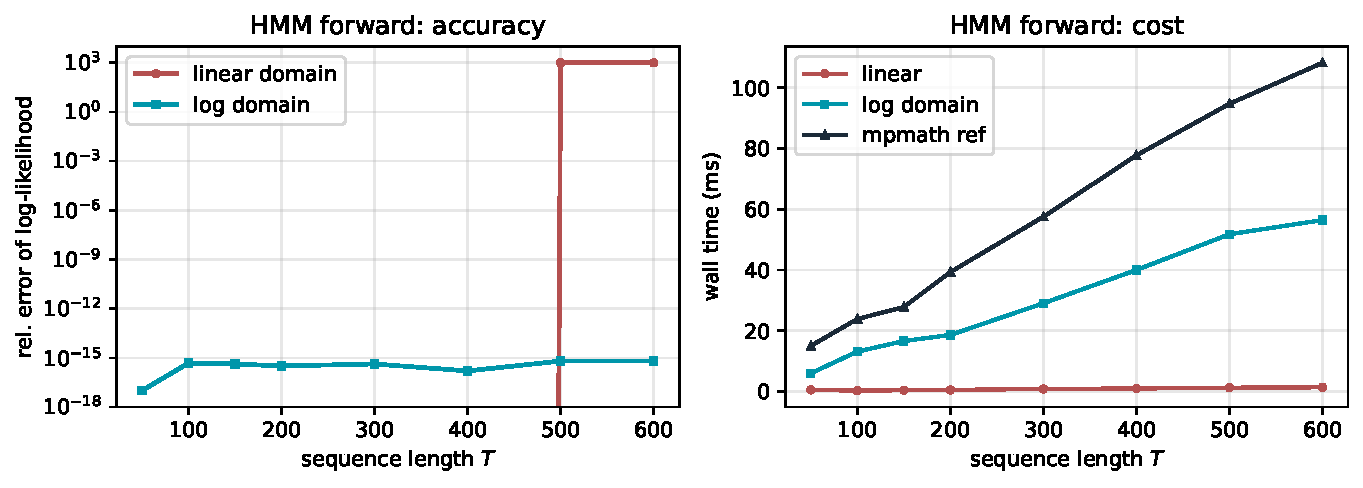
\includegraphics[width=0.96\textwidth]{figures/B6_hmm.pdf}
\caption{HMM forward log-likelihood. Left: the linear domain is exact until it
underflows ($T\gtrsim 450$, error $\to\infty$); the log domain holds at machine
precision. Right: wall time --- linear (fast but breaks), log domain (stable),
mpmath reference (slowest). Computed by \code{papers/benchmark\_hmm.py}.}
\label{fig:hmm}
\end{figure}

\noindent\emph{Reading.} The right panel reframes the trade-off in real time:
the log domain is the only option that is both \emph{correct} for all $T$ and
substantially \emph{cheaper} than the high-precision fallback. This is the
practical sweet spot the twin view predicts --- compute in the domain where the
quantity stays representable, and pay only a linear-time premium.

\section{API reference}
\label{app:api}

The decisions of this paper are one-call:

\begin{lstlisting}
from arithmetics.symbolic.twin import (
    arithmetic_task_report,   # domain comparison for a log-likelihood
    recommend_domain,         # pre-computation domain rule from data range
    total_error,              # error of a domain vs high-precision reference
    optimal_base,             # select the linearising base (loglog/semilog/...)
    op_count,                 # transcendental/arithmetic op counts
)
report = arithmetic_task_report(probs)        # dict of measured costs
base   = optimal_base(xs, ys)["optimal_base"] # e.g. 'loglog'
\end{lstlisting}

The symbolic generator and the Lie/qudit layers are reached through
\code{twin\_operation}, \code{twin\_decision}, \code{verify\_primary\_decomposition},
\code{weyl\_average}, and \code{qudit\_universality}; every object renders as a
SymPy expression, \LaTeX, Unicode, or an mpmath value.

\section{Reproducibility}
\label{app:repro}

The library ships unit tests per layer (Table~\ref{tab:tests}); the full suite
passes. All figures are regenerated by \code{papers/make\_figures.py} and the
benchmark by \code{papers/benchmark\_hmm.py}, from computed data only.

\begin{table}[ht]
\centering
\caption{Test layout (all passing).}
\label{tab:tests}
\begin{tabular}{ll}
\toprule
suite & coverage \\
\midrule
\code{test\_symbolic} & symbolic engine ($\varphi$, $\oplus_p$, $\delta$, $\zeta_p$) \\
\code{test\_twin} & transport, finite classification, counting \\
\code{test\_twin\_lie} & $SO(2),SO(3),SU(2)$ kernels, universality \\
\code{test\_twin\_decision} & class equation, normalizer orbits, Weyl $SU(2)$ \\
\code{test\_twin\_primary} & abelian primary decomposition \\
\code{test\_twin\_tasks} & arithmetic-task costs, base selection \\
\code{test\_twin\_qudit} & $SU(n)$ Weyl, Schur characters \\
\bottomrule
\end{tabular}
\end{table}

\begin{thebibliography}{9}
\bibitem{grossman} M.~Grossman, R.~Katz, \emph{Non-Newtonian Calculus},
Lee Press, 1972.
\bibitem{blanchard} P.~Blanchard, D.~J.~Higham, N.~J.~Higham, Accurately
computing the log-sum-exp and softmax functions, \emph{IMA J.\ Numer.\ Anal.}
41 (2021), 2311--2330.
\bibitem{mezzadri} F.~Mezzadri, How to generate random matrices from the
classical compact groups, \emph{Notices AMS} 54 (2007), 592--604.
\bibitem{meurer} A.~Meurer et al., SymPy: symbolic computing in Python,
\emph{PeerJ CS} 3 (2017), e103.
\bibitem{harris} C.~R.~Harris et al., Array programming with NumPy,
\emph{Nature} 585 (2020), 357--362.
\end{thebibliography}

\end{document}
